\documentclass[professionalfont]{beamer}

\usepackage{graphicx}
\usepackage{newtxtext,newtxmath}
\usepackage[backend=bibtex]{biblatex} 
\addbibresource{ref.bib}
\renewcommand*{\bibfont}{\scriptsize}

\usetheme{default}
\usecolortheme{seagull}

\setbeamertemplate{navigation symbols}{}
\setbeamertemplate{itemize item}{\textbullet} 
\setbeamertemplate{bibliography item}[text]
\setbeamertemplate{title page}{
    \begin{center}
        {\textcolor{blue}{\textbf{\fontsize{13}{14}\selectfont
        Large Language Models are Zero-Shot Reasoners}}} \\[1.5cm]
        
        {\fontsize{9}{14}\selectfont Takeshi Kojima, et al \\[0.3cm]
        The University of Tokyo, Google Research \\[0.3cm]
        NeurIPS 2022}
    \end{center}
}
% ------------------ Title ------------------

\begin{document}
\frame{\titlepage}

\begin{frame}
\begin{center}
    { \textbf{\textcolor{blue}{ {\fontsize{12}{14}\selectfont Abstract} }} }
\end{center}
\\[0.5cm]

{\fontsize{10}{14}\selectfont 
\begin{itemize}
    \item Background
    
    - Large scale \( \rightarrow \) Prompting \( \rightarrow \) CoT

    \\[0.3cm]

    \item Zero-Shot CoT

    - ``Let's think step by step"

    \\[0.3cm]

    \item Experiment

    - Zero-Shot, Few-Shot
    
    - Zero-Shot-CoT, Few-Shot-CoT
    
    - Zero-Plus-Few-Shot-CoT

    - Self-consistency

    \item Discussion

    - It is minimalist and elicits CoT
\end{itemize}
}

\end{frame}
% ------------------ Contents ------------------

\begin{frame}
\begin{center}
    { \textbf{\textcolor{blue}{{\fontsize{12}{14}\selectfont Introduction}}} }
\end{center}
\\[0.5cm]

{\fontsize{10}{14}\selectfont 
\begin{itemize}
    \item CoT's success
    
    - Step-by-step example 

    - Manually creating example is costly

    \\[0.3cm]

    \item Zero-shot CoT

    - Adding a prompt, ``Let’s think step by step"

    - Simple but strong
\end{itemize}
}

\end{frame}
% ------------------ Slide 2 ------------------

\begin{frame}
\begin{center}
    { \textbf{\textcolor{blue}{ {\fontsize{12}{14}\selectfont Zero-shot Chain of Thought} }} }
\end{center}

\begin{center}
    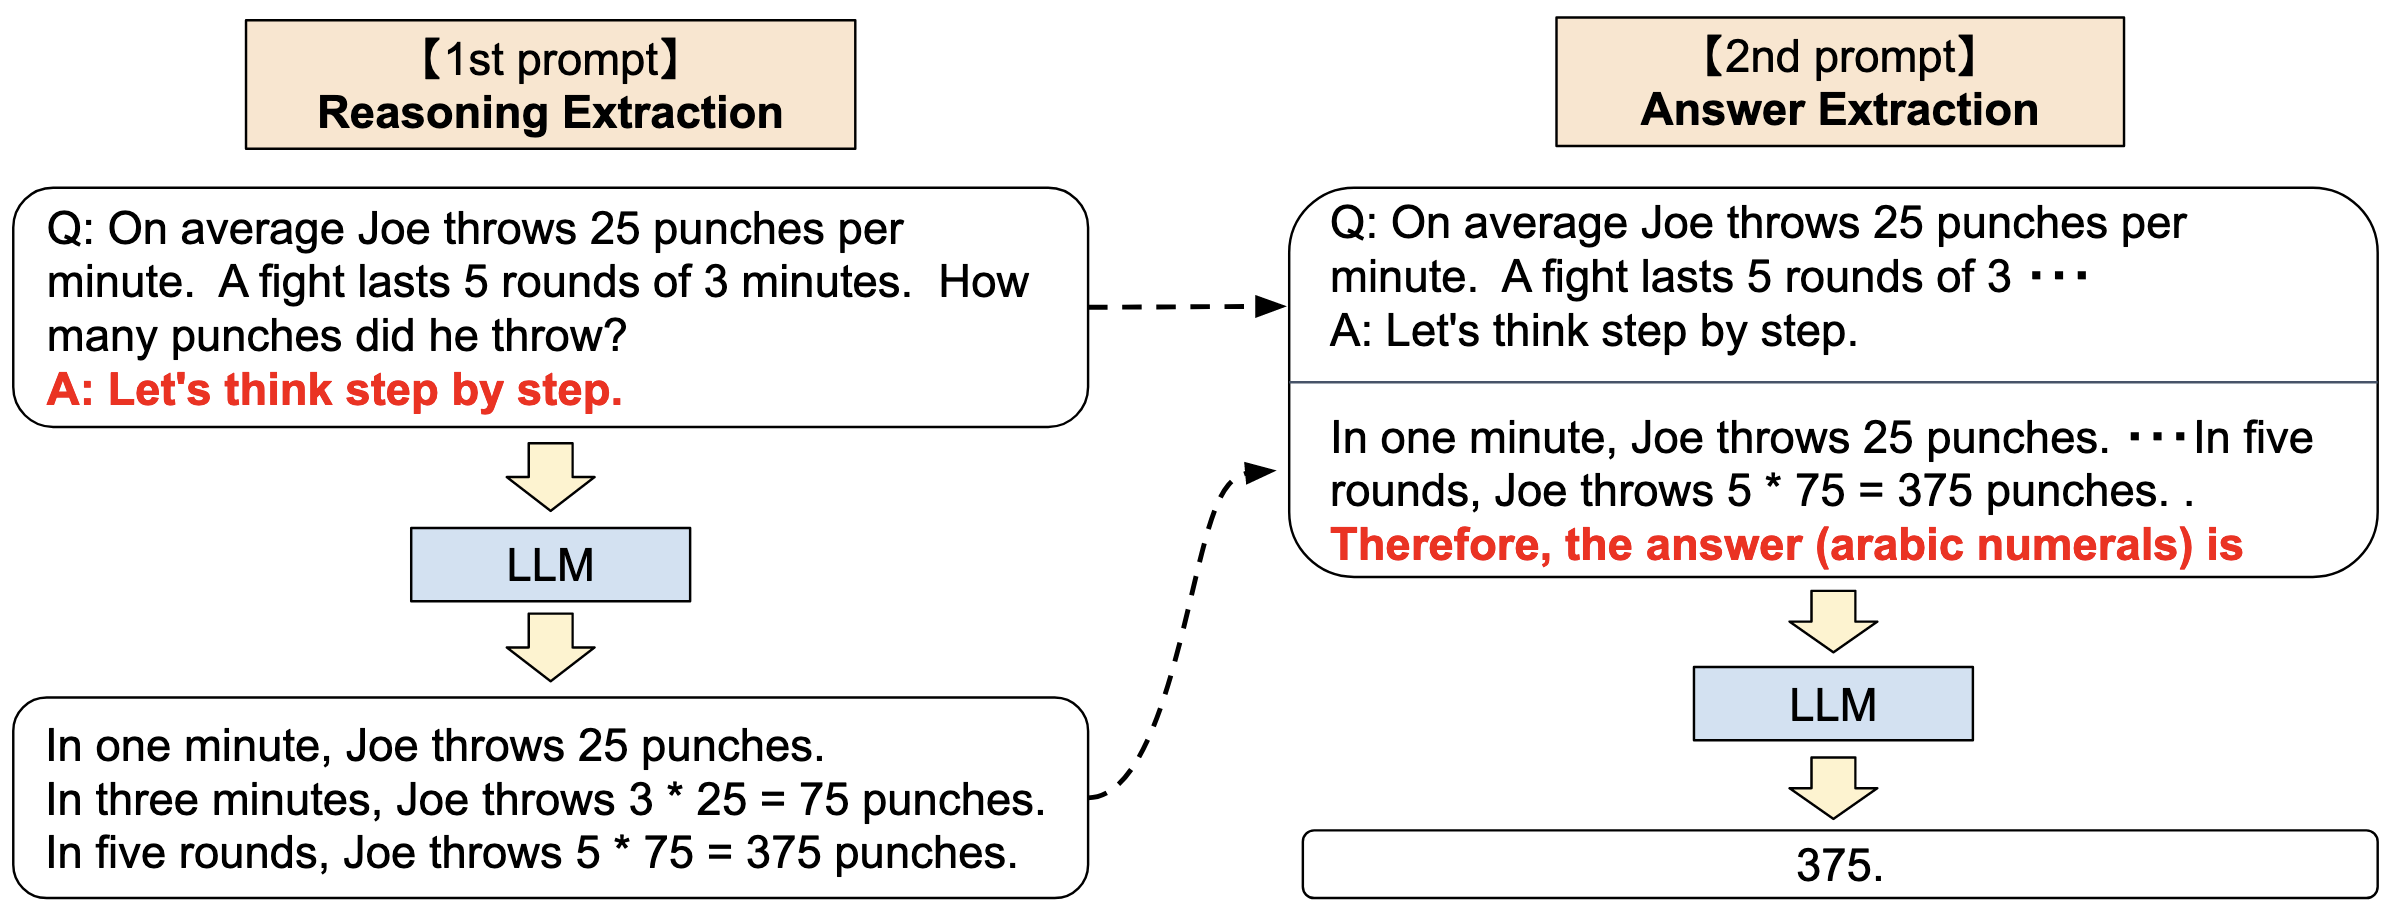
\includegraphics[width=1.0\textwidth]{figure/2.png}
\end{center}

{\fontsize{10}{14}\selectfont 
\begin{itemize}
    \item 1st prompt: reasoning extraction
    
    - Input question \( X \), reasoning trigger \( T \)

    - Prompting as ``Q: [\( X \)]. A: [\( T \)]"

    \item 2nd prompt: answer extraction

    - 1st prompt \( X' \), Generated \( Z \), answering trigger \( A \)

    - Prompting as ``[\( X' \)] [\( Z \)] [\( A \)]"
    
\end{itemize}
}

\end{frame}
% ------------------ Slide 2 ------------------

\begin{frame}

\begin{center}
    { \textbf{\textcolor{blue}{ {\fontsize{12}{14}\selectfont Experiment } }} }
\end{center}
\\[0.5cm]

{\fontsize{10}{14}\selectfont 
\begin{itemize}
    \item Tasks (Total 12 datasets)

    - Arithmetic reasoning

    - Commonsense reasoning

    - Symbolic reasoning

    - Other reasoning tasks

    \\[0.3cm]

    \item Models (Total 17 models)

    - GPT Variations (Instruct-GPT3)

    - PaLM (8B-540B)

    - Other models
\end{itemize}
}

\end{frame}
% ------------------ Slide 3 ------------------

\begin{frame}
\begin{refsection}

\begin{center}
    { \textbf{\textcolor{blue}{ {\fontsize{12}{14}\selectfont Background } }} }
\end{center}
\\[0.1cm]

{\fontsize{10}{14}\selectfont 
\begin{itemize}
    \item InstructGPT \cite{instructgpt}

    - Prompts submitted through the OpenAI API

    - Demonstrations of the desired model behavior

    - Supervised fine-tuning with the dataset

    - 1.3B InstructGPT was preferred to 175B GPT-3

    \\[0.3cm]

    \item Self-consistency \cite{self_consistency}

    - Different decoding method from greedy-one

    - Get multiple CoTs with temperature-based sampling

    - Aggregate the answers using majority voting
\end{itemize}
}

\vspace{0.3cm}
\hrule
\printbibliography

\end{refsection}
\end{frame}
% ------------------ Slide 3 ------------------

\begin{frame}

\begin{center}
    { \textbf{\textcolor{blue}{ {\fontsize{12}{14}\selectfont Zero-shot-CoT vs Zero-shot} }} }
\end{center}

\begin{center}
    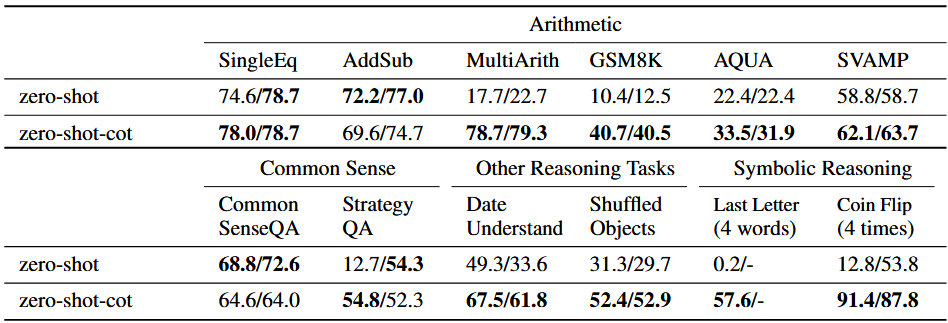
\includegraphics[width=1.0\textwidth]{table//1.png}
\end{center}

{\fontsize{10}{14}\selectfont 
\begin{itemize}
    \item GPT-3 Results
    
    - Usually, Zero-shot-CoT outperforms

    - No performance gain in commonsense reasoning

    - PaLM(540B) is expected to solve the problem
\end{itemize}
}
\end{frame}
% ------------------ Slide 4 ------------------

\begin{frame}
\begin{center}
    { \textbf{\textcolor{blue}{ {\fontsize{12}{14}\selectfont Comparison with baselines} }} }
\end{center}

\begin{center}
    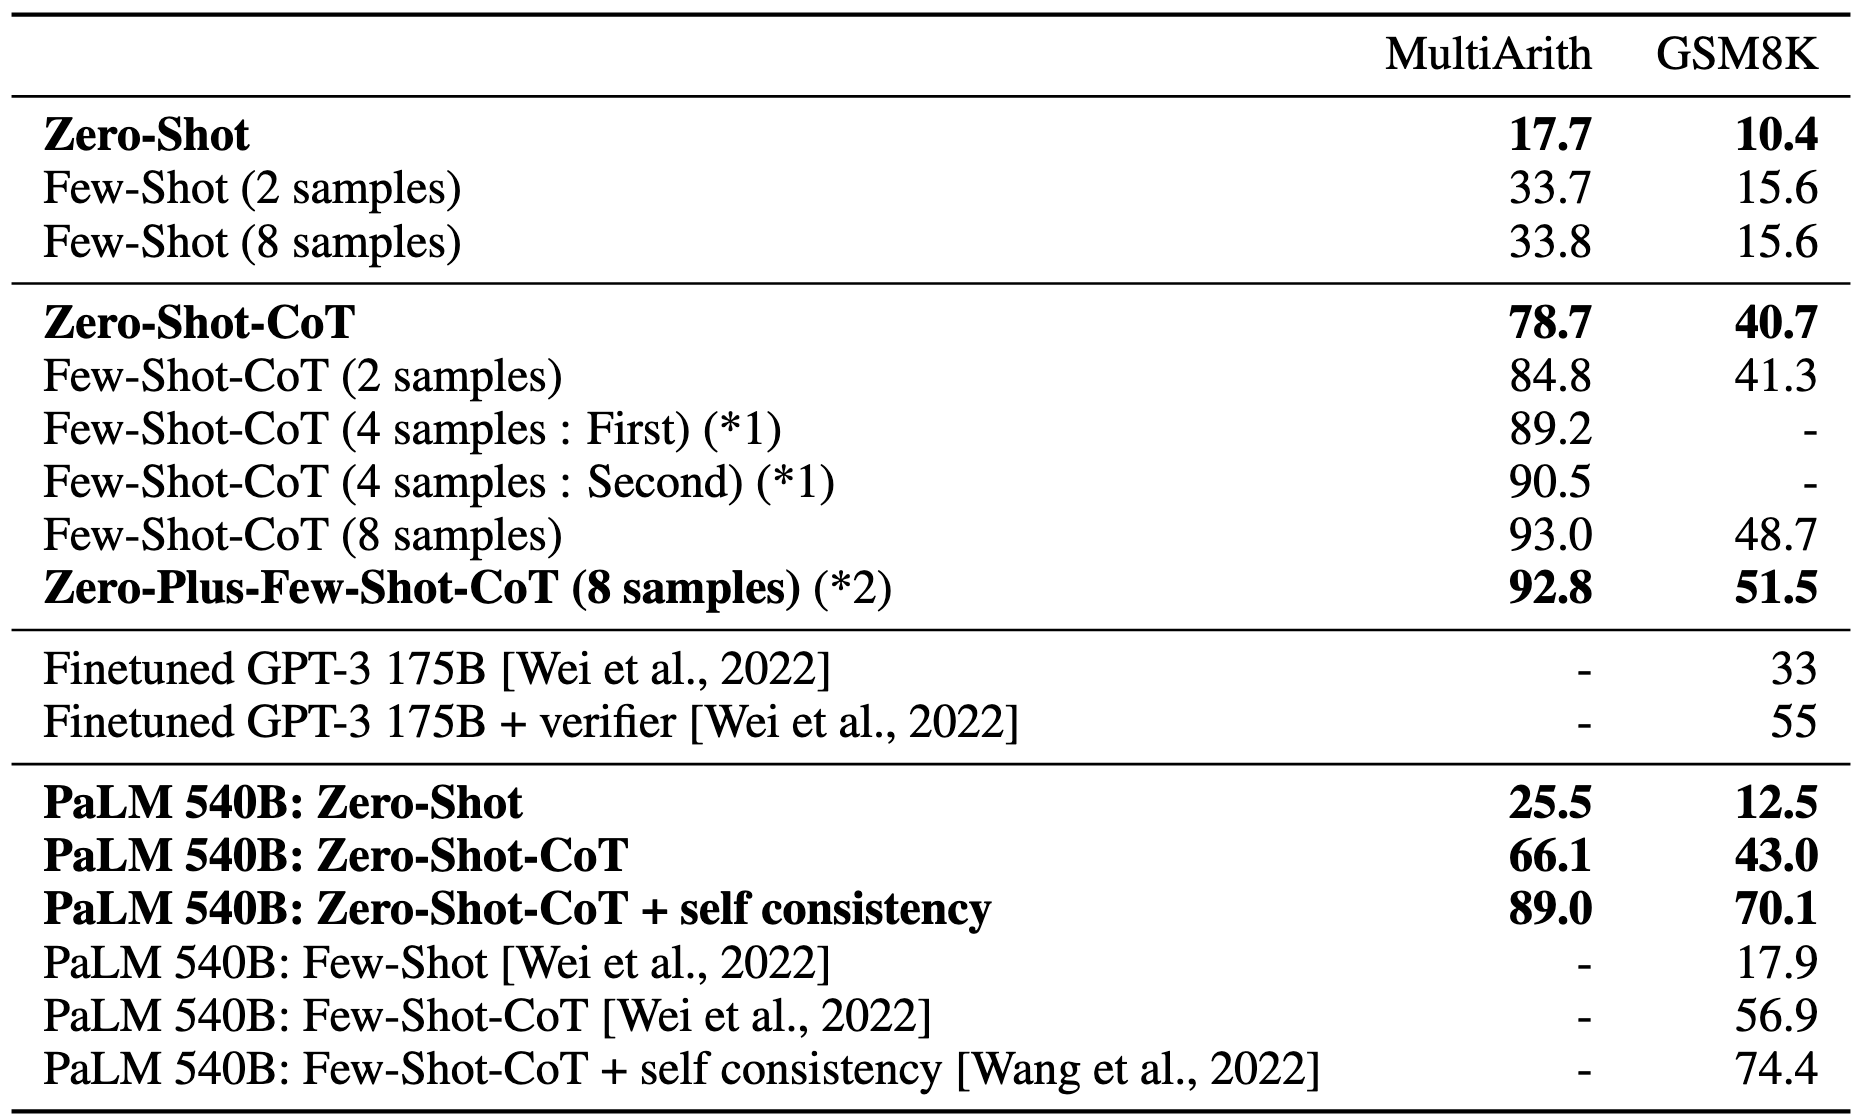
\includegraphics[width=0.9\textwidth]{table//2.png}
\end{center}

{\fontsize{10}{14}\selectfont 
\begin{itemize}
    \item Performance increases with CoT
\end{itemize}
}

\end{frame}
% ------------------ Slide 5 ------------------

\begin{frame}
\begin{center}
    { \textbf{\textcolor{blue}{ {\fontsize{12}{14}\selectfont Model scale study} }} }
\end{center}
\\[0.5cm]

\begin{center}
    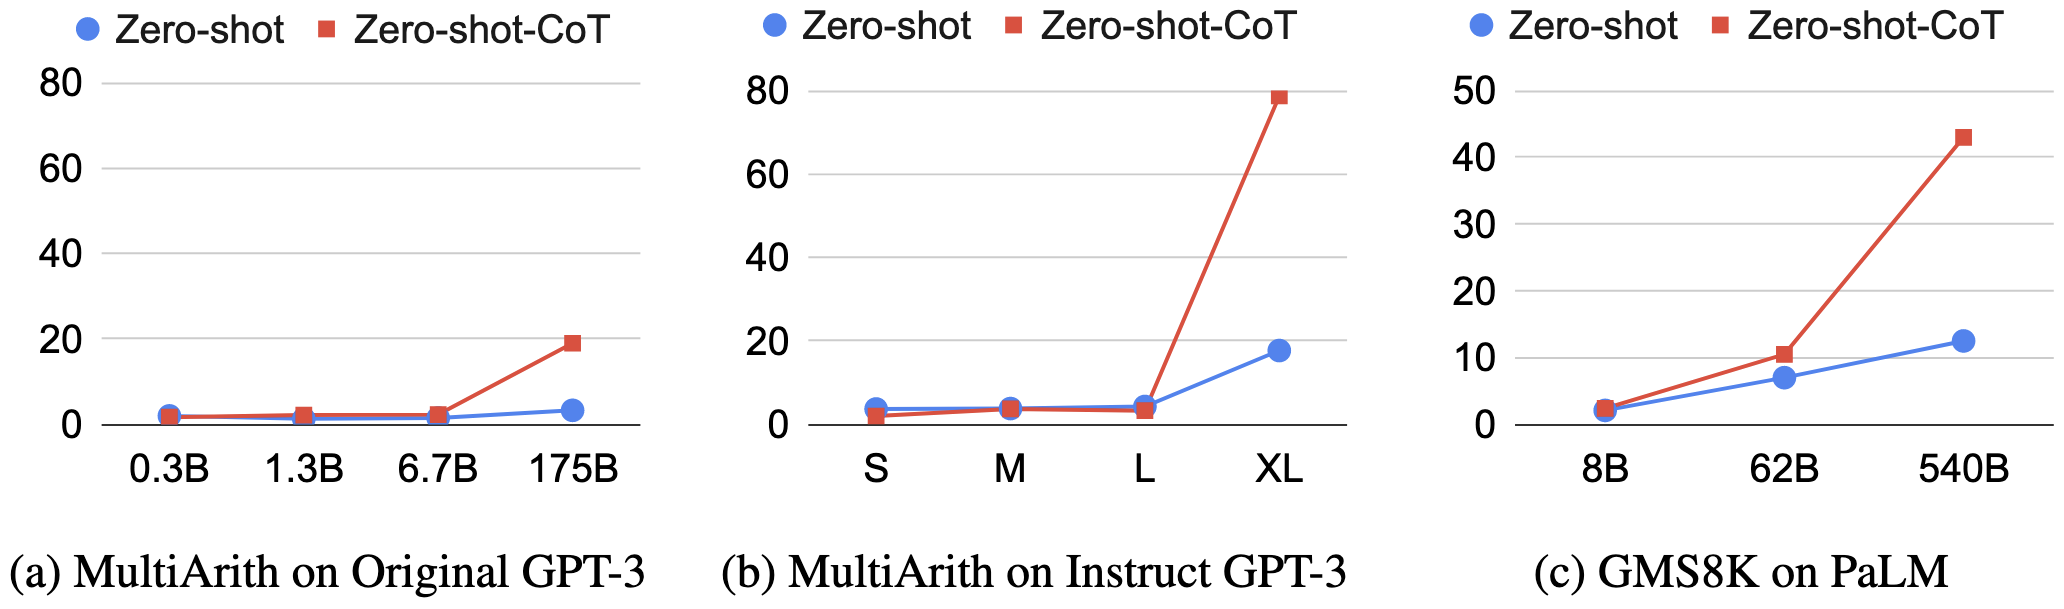
\includegraphics[width=1.0\textwidth]{figure/3.png}
\end{center}

{\fontsize{10}{14}\selectfont 
\begin{itemize}
    \item CoT is not effective when model is small

    \item Performance drastically increases as model gets bigger

\end{itemize}
}

\end{frame}
% ------------------ Slide 6 ------------------

\begin{frame}
\begin{center}
    { \textbf{\textcolor{blue}{ {\fontsize{12}{14}\selectfont Robustness study} }} }
\end{center}

\begin{center}
    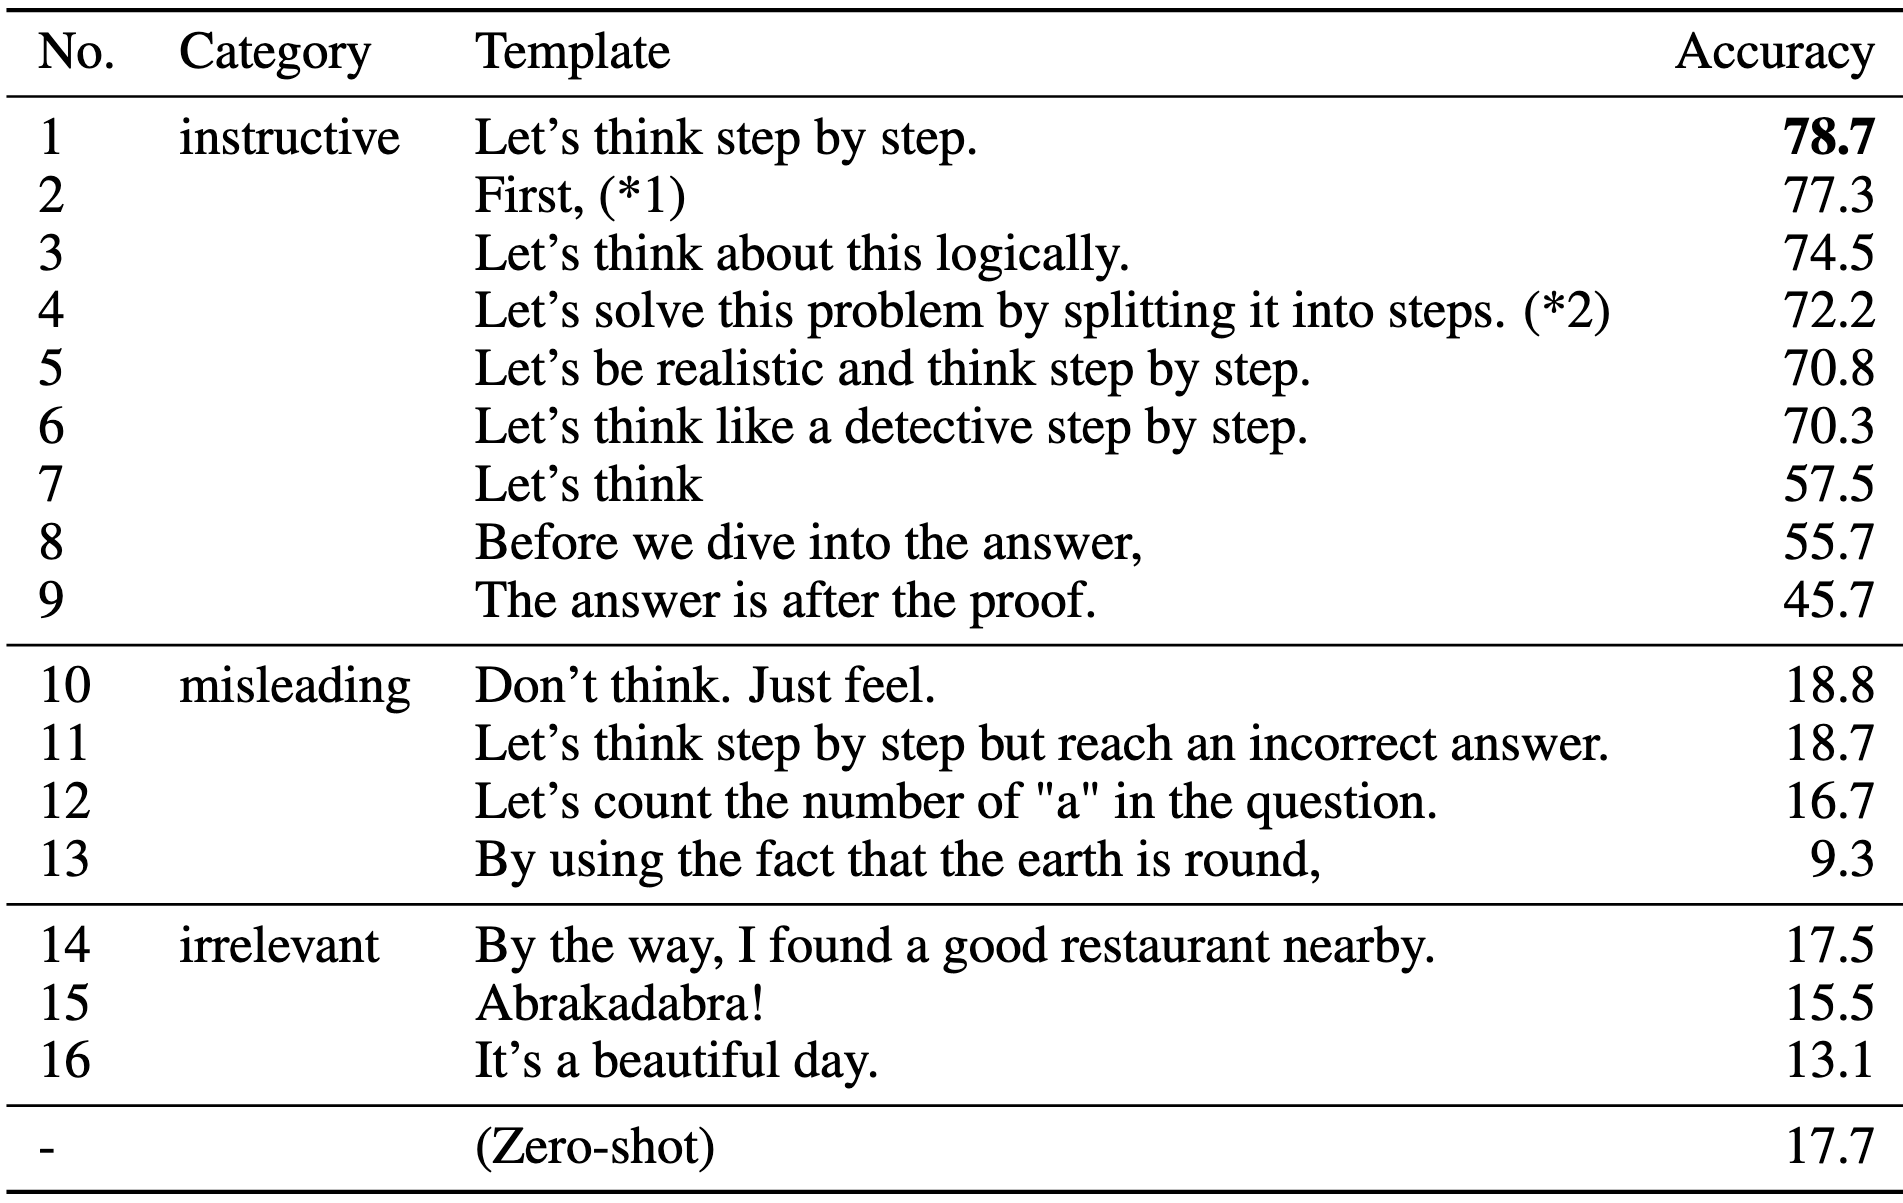
\includegraphics[width=0.9\textwidth]{table/4.png}
\end{center}

{\fontsize{10}{14}\selectfont 
\begin{itemize}
    \item Future research: Automatically creating better templates

\end{itemize}
}

\end{frame}
% ------------------ Slide 7 ------------------

\begin{frame}
\begin{center}
    { \textbf{\textcolor{blue}{ {\fontsize{12}{14}\selectfont Conclusion} }} }
\end{center}
\\[0.3cm]

{\fontsize{10}{14}\selectfont 
\begin{itemize}
    \item Reasoning Ability of LLMs

    - Performance can be increased by 3 ways orthogonally

    - Fine-tuning, Prompting, Step-by-step reasoning

    \\[0.3cm]

    \item Limitation

    - LLM amplify biases found in the training data

\end{itemize}
}

\end{frame}
% ------------------ Slide 8 ------------------


\end{document}